\section{Caution against a weak field approximation}
\label{appendix:continuum-time}

A weak field approximation for the general relativistic effects is sometimes used in the interest of making a model computationally performant. These are commonly formulated by some spherical radius $R$ outside of which relativistic effects are said to be negligible, and a flat spacetime metric is used. In \cite{cackett_modelling_2014}, $R = 100\, \rg$ for the purposes of accelerating computation when calculating lag-frequency and lag-energy spectra. However, this approximation introduces a slight error when calculating the light travel time of flux from the disc and continuum source, which has a significant effect of their computed lag-frequency spectra.

In cases where the source height above the black hole is small, the systematic error from the weak field approximation between the reflected and continuum flux is roughly equal, and therefore is negligible when the difference in arrival time is calculated, as in
\begin{equation}
    \Delta t = \tilde{t}_\text{reflected} - \tilde{t}_\text{continuum} ,
\end{equation}
where the tilde denotes the inclusion of $\delta t$ due to the weak field approximation $\tilde{t} = t - \delta t$. However, when the source height is of appreciable value, say $h > 10\rg$, then for an off axis observer the systematic error from $t_\text{wf}$ is greater for the continuum emission than for the reflected component (see Figure \ref{fig:app:weak-field-approx}), resulting in the continuum flux arriving seemingly too early. Note that $\delta t$ is dependant on the observer's position, and decreases with increasing $r_\text{obs}$. 

Figure \ref{fig:app:continuum-time} illustrates the relationship between coronal source height and $\delta t$, calculated by using the weak field approximation at different $R$ and subtracting the equivalent `true' light travel time $t$ (equivalent to $R \rightarrow \infty$). Even at $h = 100$, the continuum flux from the corona is seen to arrive significantly early.

\begin{figure}
	\centering
	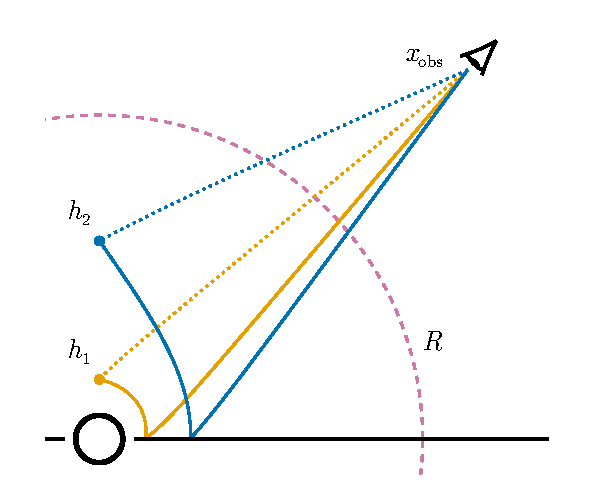
\includegraphics[width=0.80\linewidth]{figures/continuum-time.figure.pdf}
	\caption{\todo{TODO}}
	\label{fig:app:weak-field-approx}
\end{figure}

For the source heights of $h=10\, \rg$ and $h = 20 \rg$ and an observer inclination of $\theta_\text{obs} = 45^\circ$, the path length of the traject

\begin{figure}
	\centering
	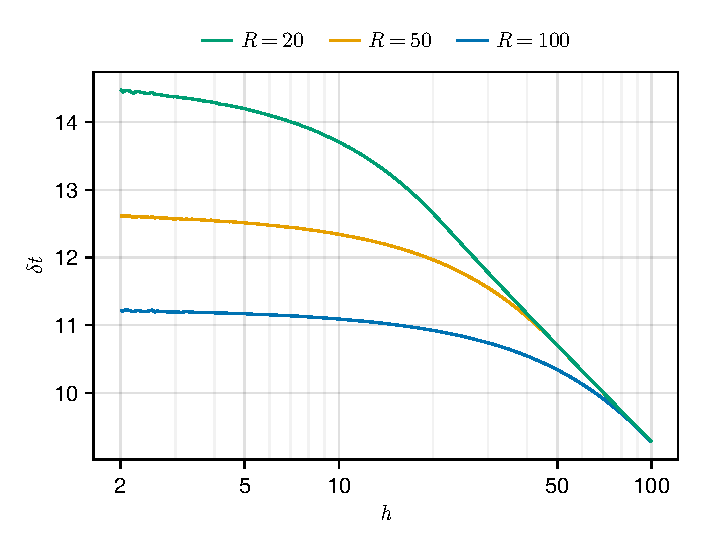
\includegraphics[width=0.98\linewidth]{figures/continuum-time.weak-field.pdf}
	\caption{\todo{TODO}}
	\label{fig:app:continuum-time}
\end{figure}